\section{Genetic Programming}
\label{sec:bg:gp}

  \emph{Genetic Programming} (GP)~\autocite{kozaGeneticProgrammingProgramming1992a,kozaGeneticProgrammingII1994,poliFieldGuideGenetic2008a,yuIntroductionEvolutionaryAlgorithms2010}
  has been carved out as a specialized subfield of EAs which emphasizes 
  evolving a collection of computer programs tailored to address specific 
  problems. While GP can be viewed as a natural evolution of 
  GAs, it distinguishes itself by its primary goal: GAs fine-tunes parameters 
  to optimize a given function, whereas GP is geared towards program induction.\footnote{%
    A more detailed definition of program induction can be found in \vref{def:program_induction}.
  }

  At their core, both GP and GA operate on similar foundations. They use a 
  population-based strategy, employ a fitness function to assess individual 
  performance, and apply genetic operators to produce new individuals. Yet, the 
  representation of individuals in GP, along with its unique genetic operators, 
  differentiates it from GA.

  \begin{remark}
    While GP is primarily a fitness-centric search in the set of computer 
    programs, its fundamental nature is optimization, echoing the core of GA.
  \end{remark}

  Within the population of GP, every individual represents a computer 
  program, built from a library of primitives, distinguished as 
  \emph{functions} and \emph{terminals}. One way to represent this is as a 
  composite pattern where functions are internal nodes, and terminals are the leaves. This structure is commonly referred to as an abstract syntax tree (AST). For a visual representation, refer to \vref{fig:composite_pattern}.

  \begin{figure}[ht!]
    \centering
    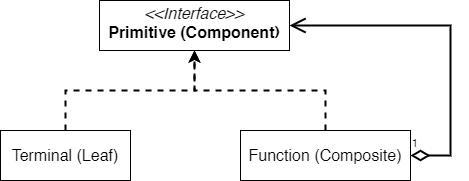
\includegraphics[width=0.4\textwidth]
      {img/theoretical_framework/GP Composite.png}
    \caption{
      Representation of GP individuals as a composite structure.
    }
    \label{fig:composite_pattern}
  \end{figure}

  The GP algorithm, delineated in \vref{lst:bg:gp:algorithm}, bears structural 
  resemblance to the GA algorithm. The key differentiator rests in the specific 
  genetic operations tailored for GP.

  \begin{code}{
    Structural blueprint of the Genetic Programming algorithm, underscoring its 
    architectural alignment with the Genetic Algorithm.
  }{label=lst:bg:gp:algorithm}{kotlin}
    var population = recursively construct random programs
    population.forEach { it -> execute it then evaluate it }
    while (termination criteria is not met) {
      val survivors = select survivors from population
      val parents = select parents from population
      val offspring = alter parents
      offspring.forEach { it -> execute it then evaluate it }
      population = survivors + offspring
    }
    return fittest from population
  \end{code}

  In the following sections, we will delve into the key components of the GP 
  algorithm, clarifying these concepts with practical examples.

\subimport{representation/}{_representation.index.tex}
\subimport{initialization/}{Initialization.tex}
\subimport{selection}{Selection.tex}
\subimport{./variation/}{_variation.index.tex}
\subimport{./}{Generalization.tex}
